%\begin{figure}[h!]
%    \centering
%    \includegraphics[width=14cm, height= 7.5cm]{.png}
%    \caption{}
%    \label{fig:}
%\end{figure}

%-------------------------------------------------------------------------%
\section{Performance of the classifiers}
%-------------------------------------------------------------------------%
%\subsection{Benchmark 1: \texorpdfstring{$\Tilde{t} = 1.2$}{ } TeV and \texorpdfstring{$\Tilde{\chi}_1^0 = 600$}{ } GeV}
An initial measure to visually understand how our classifiers have performed, a simple Receiver operating characteristic (ROC) curve can be constructed. A ROC curve shows the distribution of the predicted values given between 0 and 1, as a function of FP rate versus TP rate. This allows us to understand how much error we are willing to accept/reject for a given model, where we can produce histograms to observe where the optimum cut-off may be (see Figures \ref{fig:dist_bm1}-\ref{fig:dist_bm_in}. The ROC curve produced for all four benchmark data is presented in Figure \ref{fig:ROC} showing excellent performance across. As expected, however, the benchmark set corresponding to mass parameters within the exclusion curve (benchmark4: $\Tilde{t} = 750$ GeV and $\Tilde{\chi}_1^0 = 1$ GeV) performed the worst amongst the four due to the smaller mass difference between the stops and neutralinos. We also note that the datasets performed better as the mass difference became larger, which is also an expected behavior as the larger mass difference creates more energetic (anti)tops, consequently, more missing energy. This allowed the classifier to pick up such signatures easily, and we suspect that the missing energy's magnitude is the most influential variable the classifier has used when performing its splits. \\


\begin{figure}[htbp]
    \centering
    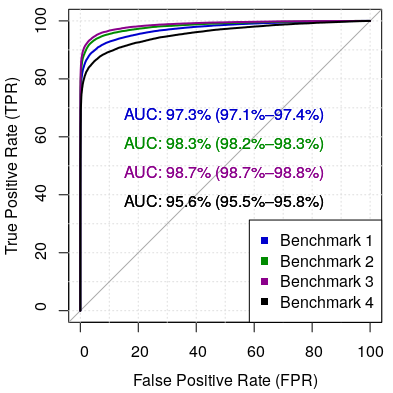
\includegraphics[width=0.4\linewidth]{ROC_curve.png}
    \caption{ROC curve for all 4 benchmark points. The forth benchmark corresponding to masses within the exclusion curve performed least well, where the remaining three performed slightly better when the mass difference between the stops and neutralinos became larger.}
    \label{fig:ROC}
\end{figure} 

Although the Area-under-the-curve (AUC) value is given in Figure \ref{fig:ROC}, it is maximized and does not directly represent the accuracy of our models. The accuracy of our models can be obtained by setting a cut-off to our predictions i.e. a number between 0 and 1. The closer the value is to 1 the lower the accuracy, but deliberately obtaining a high accuracy by setting a smaller value is also conter-intuitive as the Signal-to-Noise Ratio (SBR) will be smaller. Through various trials in cut-off values, it was determined for all four datasets that 0.75 is the optimal value to satisfy both high accuracy and high SBR. \\

For the benchmark point $\Tilde{t} = 1.2$ TeV and $\Tilde{\chi}_1^0 = 600$ GeV, the classifier performed quite well, producing a result of above $90\%$ accuracy. It is expected that the classifier performed less accurately when dealing with signal-like events. It correctly identified a smaller portion of true signal events and incorrectly classified more signal-like background events, as seen in Table \ref{tab:Values1}. The number of expected number of signal is significantly less than the expected number of background, producing an AMS value of 0.1. Considering the definition of AMS given in Section \ref{sec:metrics}, it supports the exclusion limit in Figure \ref{fig:limits}. \\

\noindent\begin{minipage}{\textwidth}
\centering
  \begin{minipage}[htbp]{0.6\textwidth}
    \centering
    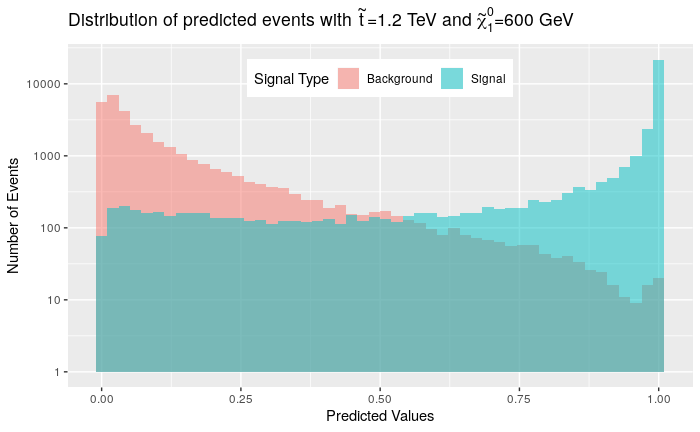
\includegraphics[width=\linewidth]{bm1_distribution.png}
    \captionof{figure}{Distribution of predicted background (pink) and signal (blue) events. The signal has a sharp drop-off at higher cut-off values unlike the background steadily, almost linearly, decreasing in number toward higher values. Note that y-axis is in a $\log_{10}$ scale.}
    \label{fig:dist_bm1}
  \end{minipage}
  \hfill
  \begin{minipage}[htbp]{0.39\textwidth}
        \centering
        \begin{tabular}{c|c} 
        \toprule
        Metric & Proportion \\
        \midrule
        \rowcolor{gray!6} TP & $42.0 \%$ \\
        TN & $49.4 \%$ \\
        \rowcolor{gray!6} FP & $0.6 \%$\\
        FN & $8.0 \%$ \\
        \rowcolor{gray!6} Accuracy & $91.4 \pm 0.2 \%$ \\
        \midrule
        $b$ & $388$ \\
        \rowcolor{gray!6} $s$ & $2$ \\
        SBR & $0.52\%$\\
        \rowcolor{gray!6} AMS & $0.1$ \\
        \bottomrule
        \end{tabular}
        \captionof{table}{Proportion of correctly and incorrectly classified points with the number of expected events calculated with Equation (\ref{eq:N}). The ratio, SBR, and AMS (Equation (\ref{eq:AMS})) were also calculated.} 
        \label{tab:Values1}
    \end{minipage}
\end{minipage}
\hfill \break
%-------------------------------------------------------------------------%
%\subsection{Benchmark 2: \texorpdfstring{$\Tilde{t} = 1.225$}{ } TeV and \texorpdfstring{$\Tilde{\chi}_1^0 = 400$}{ } GeV}

\noindent\begin{minipage}{\textwidth}
\centering
  \begin{minipage}[htbp]{0.6\textwidth}
    \centering
    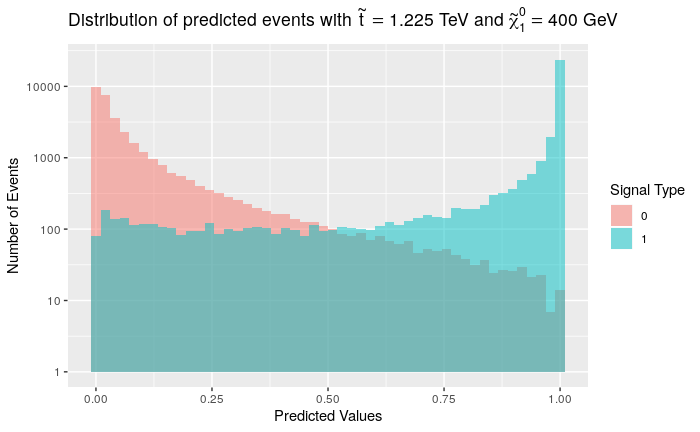
\includegraphics[width=\linewidth]{bm2_distribution.png}
    \captionof{figure}{Distribution of predicted background (pink) and signal (blue) events. The signal has a sharp drop-off at higher cut-off values unlike the background steadily, almost linearly, decreasing in number toward higher values. Note that y-axis is in a $\log_{10}$ scale.}
    \label{fig:dist_bm2}
  \end{minipage}
  \hfill
  \begin{minipage}[htbp]{0.39\textwidth}
        \centering
        \begin{tabular}{c|c} 
        \toprule
        Metric & Proportion \\
        \midrule
        \rowcolor{gray!6} TP & $43.8 \%$ \\
        TN & $49.5 \%$ \\
        \rowcolor{gray!6} FP & $0.5 \%$\\
        FN & $6.2 \%$ \\
        \rowcolor{gray!6} Accuracy & $93.3 \pm 0.2 \%$ \\
        \midrule
        $b$ & $362$ \\
        \rowcolor{gray!6} $s$ & $6$ \\
        SBR & $1.7\%$\\
        \rowcolor{gray!6} AMS & $0.31$ \\
        \bottomrule
        \end{tabular}
        \captionof{table}{Proportion of correctly and incorrectly classified points with the number of expected events calculated with Equation (\ref{eq:N}). The ratio, SBR, and AMS (Equation (\ref{eq:AMS})) were also calculated.} 
        \label{tab:Values2}
    \end{minipage}
\end{minipage}
\hfill \hfill \break
%-------------------------------------------------------------------------%
%\subsection{Benchmark 3: \texorpdfstring{$\Tilde{t} = 1.25$}{ } TeV and \texorpdfstring{$\Tilde{\chi}_1^0 = 100$}{ } GeV}

\noindent\begin{minipage}{\textwidth}
\centering
  \begin{minipage}[htbp]{0.6\textwidth}
    \centering
    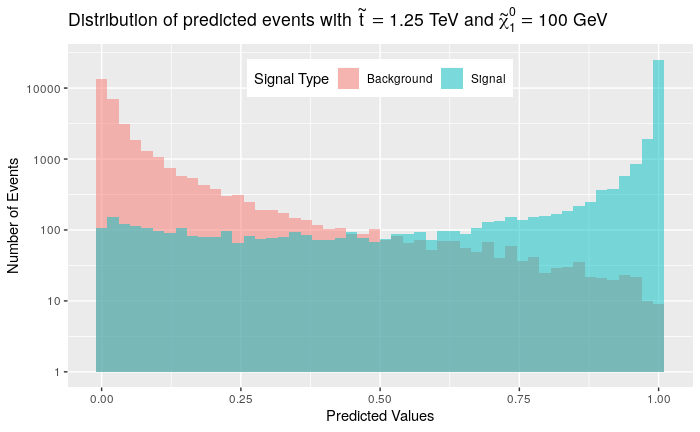
\includegraphics[width=\linewidth]{bm3_distribution.png}
    \captionof{figure}{Distribution of predicted background (pink) and signal (blue) events. The signal has a sharp drop-off at higher cut-off values unlike the background steadily, almost linearly, decreasing in number toward higher values. Note that y-axis is in a $\log_{10}$ scale.}
    \label{fig:dist_bm3}
  \end{minipage}
  \hfill
  \begin{minipage}[htbp]{0.39\textwidth}
        \centering
        \begin{tabular}{c|c} 
        \toprule
        Metric & Proportion \\
        \midrule
        \rowcolor{gray!6} TP & $44.9 \%$ \\
        TN & $49.5 \%$ \\
        \rowcolor{gray!6} FP & $0.5 \%$\\
        FN & $5.1 \%$ \\
        \rowcolor{gray!6} Accuracy & $94.4 \pm 0.2 \%$ \\
        \midrule
        $b$ & $323$ \\
        \rowcolor{gray!6} $s$ & $11$ \\
        SBR & $3.4\%$\\
        \rowcolor{gray!6} AMS & $0.6$ \\
        \bottomrule
        \end{tabular}
        \captionof{table}{Proportion of correctly and incorrectly classified points with the number of expected events calculated with Equation (\ref{eq:N}). The ratio, SBR, and AMS (Equation (\ref{eq:AMS})) were also calculated.} 
        \label{tab:Values3}
    \end{minipage}
\end{minipage}
\hfill\break
%-------------------------------------------------------------------------%
%\subsection{Benchmark 4: \texorpdfstring{$\Tilde{t} = 750$}{ } GeV and \texorpdfstring{$\Tilde{\chi}_1^0 = 1$}{ } GeV}

\noindent\begin{minipage}{\textwidth}
  \centering
  \begin{minipage}[htbp]{0.6\textwidth}
    \centering
    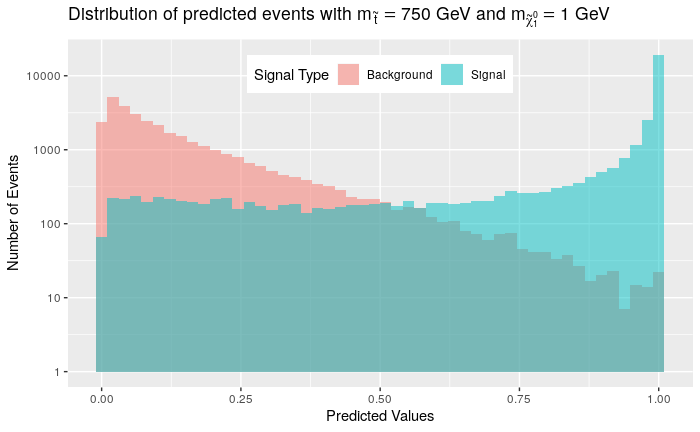
\includegraphics[width=\linewidth]{bm_In_distribution.png}
    \captionof{figure}{Distribution of predicted background (pink) and signal (blue) events. The signal has a sharp drop-off at higher cut-off values unlike the background steadily, almost linearly, decreasing in number toward higher values. Note that y-axis is in a $\log_{10}$ scale.}
    \label{fig:dist_bm_in}
  \end{minipage}
  \hfill
  \begin{minipage}[htbp]{0.39\textwidth}
        \centering
        \begin{tabular}{c|c} 
        \toprule
        Metric & Proportion \\
        \midrule
        \rowcolor{gray!6} TP & $39.4 \%$ \\
        TN & $49.6 \%$ \\
        \rowcolor{gray!6} FP & $0.4 \%$\\
        FN & $10.6 \%$ \\
        \rowcolor{gray!6} Accuracy & $89.0 \pm 0.2 \%$ \\
        \midrule
        $b$ & $343$ \\
        \rowcolor{gray!6} $s$ & $54$ \\
        SBR & $15.7\%$\\
        \rowcolor{gray!6} AMS & $2.8$ \\
        \bottomrule
        \end{tabular}
        \captionof{table}{Proportion of correctly and incorrectly classified points with the number of expected events calculated with Equation (\ref{eq:N}). The ratio, SBR, and AMS (Equation (\ref{eq:AMS})) were also calculated.} 
        \label{tab:Values_in}
    \end{minipage}
\end{minipage}
\hfill\break

\begin{table}[htbp]
    \centering
    \begin{tabular}{c||c|c}
        \toprule
        Metric & I.L. = $137\text{fb}^{-1}$ & I.L. = $35.9\text{fb}^{-1}$ \\
        \midrule
        \rowcolor{gray!6} $b$ & $343$ & $90$ \\
        $s$ & $54$ & $14$\\
        \rowcolor{gray!6} SBR & $15.7\%$ & $15.6\%$\\
        AMS & $2.8$ & $1.37$ \\
        \bottomrule
    \end{tabular}
    \caption{A table comparing values obtained with two different values for the integrated luminosity (I.L.), $137\text{fb}^{-1}$ and $35.9\text{fb}^{-1}$, within the mass parameter $\Tilde{t} = 750$ GeV and $\Tilde{\chi}_1^0 = 1$ GeV. Although the AMS values differ, the SBR is almost identical, showing that the sensitivity is no different across varying luminosity.}
    \label{tab:valsComp}
\end{table}
\hfill\break

The AMS value of 0.75 obtained by this benchmark is less than but close to the value found by Roxlo and Reece \cite{roxlo2018opening} which was 1.72. This is a reassuring result, as the exclusion limit shows that indeed this point is unlikely to be the mass parameters for both the stop and the neutralino. \\

XGBoost has an additional useful feature that calculates the \textit{feature importance} according to the \textit{Gain}, \textit{Cover} and \textit{Frequency} of each variable fed into building the classifiers \cite{xgboost}. We have used the metric `Gain' as it corresponds to the contribution of each variable based on the total gain they had when performing splits. We plot the variables accordingly, shown in Figure \ref{fig:imps} below. \\

\begin{figure}[htbp]
\centering
  \begin{minipage}[htbp]{0.45\textwidth}
    \centering
    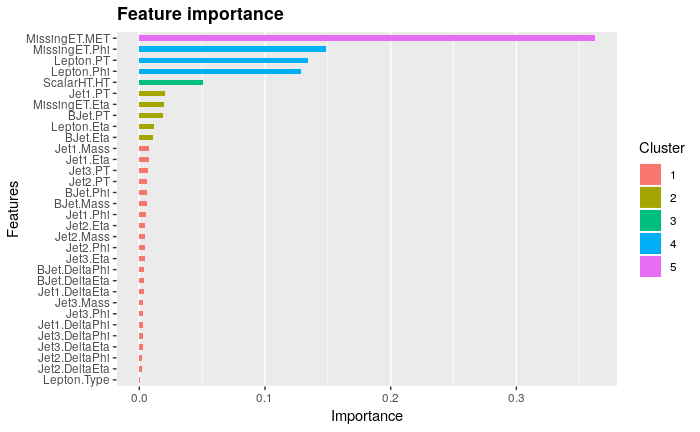
\includegraphics[width=\linewidth, keepaspectratio=true]{imp1.png}
    %\captionof{figure}{Feynman diagram of the leading order background process $pp \rightarrow t \Bar{t} \rightarrow b\Bar{b}l^{+}jj\cancel{\it{E}}_{T} $.}
    \label{fig:imp1}
  \end{minipage}
  \hfill
  \begin{minipage}[htbp]{0.45\textwidth}
    \centering
    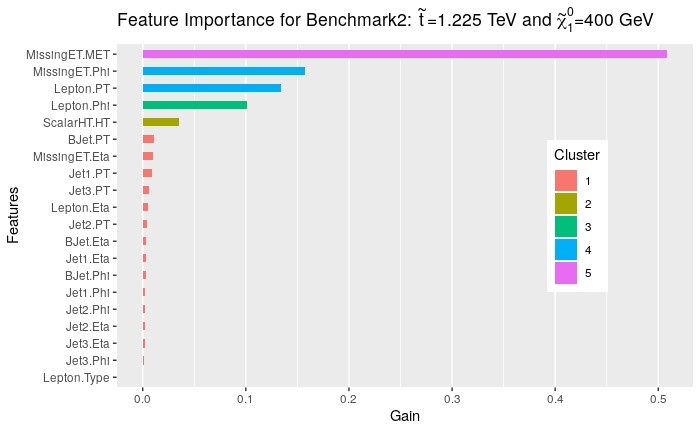
\includegraphics[width=\linewidth, keepaspectratio=true]{imp2.png}
    %\captionof{figure}{Feynman diagram of the leading order signal process $ pp \rightarrow \Tilde{t}\Tilde{t^*} \rightarrow t \Bar{t} \chi^0_1\chi^0_1 \rightarrow b\Bar{b}l^{+}jj\cancel{\it{E}}_{T} $ where the final states are identical to that of the background in Figure \ref{fig:bkrdFeyn}.}
    \label{fig:imp2}
  \end{minipage}
  \hfill
  \begin{minipage}[htbp]{0.45\textwidth}
    \centering
    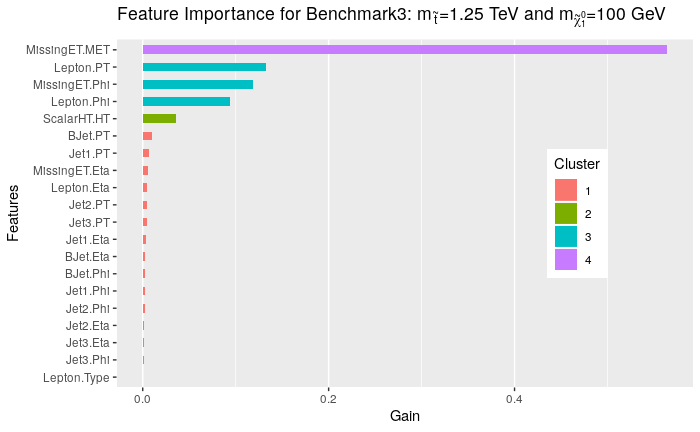
\includegraphics[width=\linewidth, keepaspectratio=true]{imp3.png}
    %\captionof{figure}{Feynman diagram of the leading order background process $pp \rightarrow t \Bar{t} \rightarrow b\Bar{b}l^{+}jj\cancel{\it{E}}_{T} $.}
    \label{fig:imp3}
  \end{minipage}
  \hfill
  \begin{minipage}[htbp]{0.45\textwidth}
    \centering
    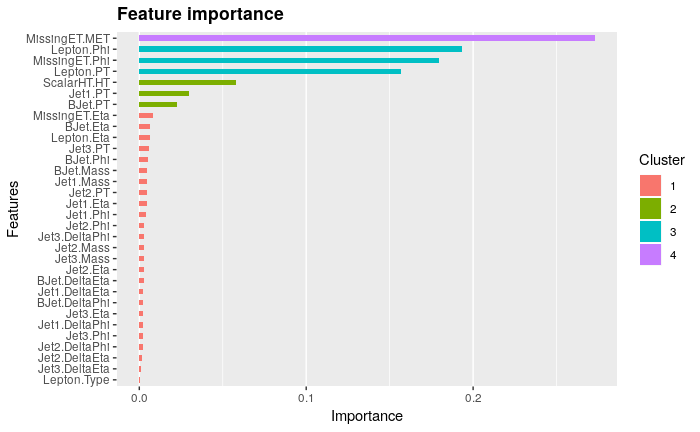
\includegraphics[width=\linewidth, keepaspectratio=true]{imp_in.png}
    %\captionof{figure}{Feynman diagram of the leading order signal process $ pp \rightarrow \Tilde{t}\Tilde{t^*} \rightarrow t \Bar{t} \chi^0_1\chi^0_1 \rightarrow b\Bar{b}l^{+}jj\cancel{\it{E}}_{T} $ where the final states are identical to that of the background in Figure \ref{fig:bkrdFeyn}.}
    \label{fig:imp_n}
  \end{minipage}
  \caption{The feature importance for all four benchmark points ordered from top-left to bottom-right. All four classifiers considers $\cancel{\it{E}}_{T}$ the most important feature, followed by the $\phi$ component of $\cancel{\it{E}}_{T}$ and the lepton as well as the lepton's $p_T$, not necessarily in this order. Furthermore the fifth most important variable is $H_T$ opposed to a particular jet's $p_T$. The clustering helps us to undestand the which variables were grouped together when considering a split. (??  Unsure about this explanation as I cannot find a good reference on the internet for it.)}
  \label{fig:imps}
\end{figure}

From the bar-plots shown in Figure \ref{fig:imps}, we notice that the algorithm had the highest contribution from the variable $\cancel{\it{E}}_{T}$ thus making it the most important. This is to be expected as we know that the neutralinos contribute to $\cancel{\it{E}}_{T}$ but also the SM neutrinos due to the highly energetic top quarks produced in our signal events. The next highest contributors were the $\phi$ components of $\cancel{\it{E}}_{T}$ and the lepton as well as its $p_T$, followed by the hadronic energy $H_T$. These five variables were consistently the top-five contributors to the algorithm and observing the grouping (noted as clusters in the legend), we can infer that the in particular, that the $\phi$ components of $\cancel{\it{E}}_{T}$ and the lepton have some sort of correlation with an occasional contribution from the lepton's $p_T$. We also observe that the $p_T$ of the $b$-jet and the remaining jet with highest $p_T$ (referred to as jet-1 henceforth) occasionally have slight contribution to the algorithm, with the remaining variables considered almost irrelevant consistently.
%-------------------------------------------------------------------------%
\section{Data Visualisation using \textit{tourr}}

In this section, I would like to show how data visualisation could be useful in helping understand new physics beyond the SM better. By creating a two-dimensional projection of the data entailing of higher dimensions (i.e. many variables), we can observe the distribution of data points in such a projection. The \textit{tourr} package from R \cite{tourr} is an ideal program for such a task, producing interesting results. The projected tour requires an index to minimize the distance between certain points in a dataset, in which we chose to utilize the \textit{alpha-hull} index. A corresponding basis is generated with each projection, and the algorithm will search through potentially more optimal projections through each iteration. NEED TO EXPLAIN ABOUT ALPHA INDEX A BIT AND SHOW SOME SPLOTS AND TALK ABOUT THE PHYSICS WE CAN INTERPRET FROM IT.


%  \begin{table}[htbp]
%        \centering
%        \begin{tabular}{c||c|c|c|c}
%        \toprule
%        &\multicolumn{1}{c|}{\bfseries Benchmark1}  &
%        \multicolumn{1}{c|}{\bfseries Benchmark2}  &
%        \multicolumn{1}{c|}{\bfseries Benchmark3} &
%        \multicolumn{1}{c}{\bfseries Benchmark4} \\
%        \midrule
        %----------------------------------%
%        \textbf{Metric} & Proportion & Proportion & Proportion & Proportion \\
%        \midrule
%        \rowcolor{gray!6} TP & $42.0 \%$ & $43.8 \%$ & $44.9 \%$ & $39.3 \%$ \\
%        TN & $49.4 \%$ & $49.5 \%$ & $49.4 \%$ & $49.5 \%$ \\
%        \rowcolor{gray!6} FP & $0.6 \%$ & $0.5 \%$ & $0.6 \%$ & $0.5 \%$\\
%      FN & $8.0 \%$ & $6.2 \%$ & $5.1 \%$ & $10.7 \%$ \\
%        \rowcolor{gray!6} Accuracy & $91.3 \pm 0.2 \%$ & $93.3 \pm 0.2 \%$ & $94.2 \pm 0.2 \%$ & $88.8 \pm 0.2 \%$ \\
%        \midrule
%        $b$ & $403$ & $368$ & $371$ & $382$ \\
%        \rowcolor{gray!6} $s$ & $2$ & $46$ & $11$ & $53$ \\
%        SBR & $0.5\%$ & $12.5\%$ & $3.0\%$ & $13.9\%$\\
%        \rowcolor{gray!6} AMS & $0.098$ & $2.32$ & $0.56$ & $2.62$ \\
%        \bottomrule
%        \end{tabular}
%        \caption*{Proportion of important values obtained in the four benchmark parameters.}
%    \end{table}